\documentclass[tikz,border=8pt]{standalone}
\usepackage{fontspec}\setmainfont{TeX Gyre Heros}
\usetikzlibrary{arrows.meta}
\definecolor{c64blue}{RGB}{44,41,177}\definecolor{cac}{RGB}{200,150,60}
\definecolor{bad}{RGB}{170,60,60}
\begin{document}
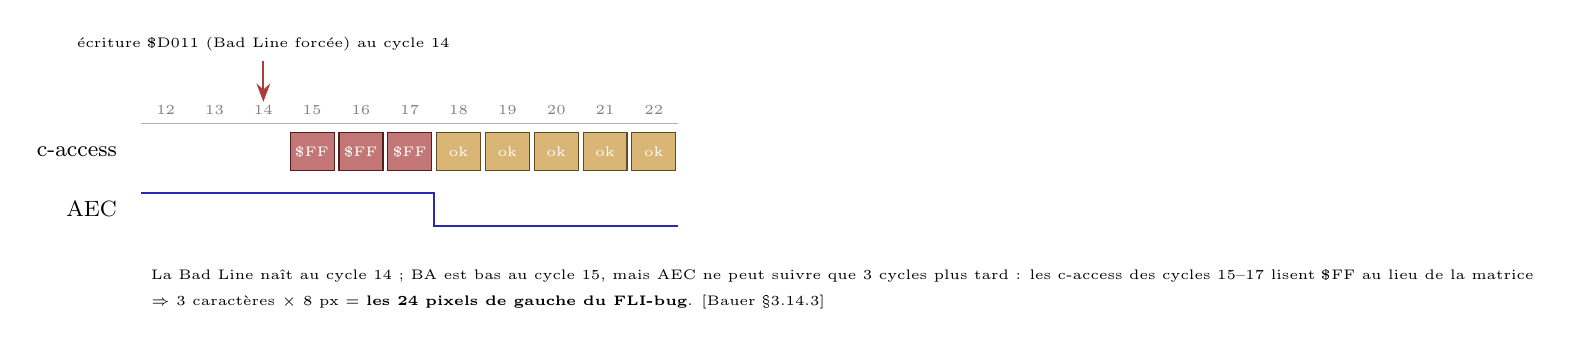
\begin{tikzpicture}[x=0.62cm,y=0.7cm,font=\footnotesize]
% axe cycles 12..22
\foreach \c in {12,...,22}{ \node[gray] at (\c-12,2.3) {\tiny\c}; }
\draw[gray!60] (-0.5,2.05) -- (10.5,2.05);
% ecriture $D011 au cycle 14
\draw[-{Stealth},thick,bad] (2,3.2) -- (2,2.45);
\node[above] at (2,3.2) {\tiny écriture \$D011 (Bad Line forcée) au cycle 14};
% c-access
\foreach \c/\ok in {15/0,16/0,17/0,18/1,19/1,20/1,21/1,22/1}{
  \ifnum\ok=0
    \draw[fill=bad!70,draw=bad!50!black] (\c-12-0.45,1.2) rectangle ++(0.9,0.7);
    \node[white] at (\c-12,1.55) {\tiny\$FF};
  \else
    \draw[fill=cac!70,draw=cac!50!black] (\c-12-0.45,1.2) rectangle ++(0.9,0.7);
    \node[white] at (\c-12,1.55) {\tiny ok};
  \fi
}
\node[anchor=east] at (-0.8,1.55) {c-access};
% AEC
\node[anchor=east] at (-0.8,0.5) {AEC};
\draw[thick,c64blue] (-0.5,0.8) -- (5.5,0.8) -- (5.5,0.2) -- (10.5,0.2);
\node[align=left,anchor=north west] at (-0.5,-0.4) {\tiny La Bad Line naît au cycle 14 ; BA est bas au cycle 15, mais AEC ne peut suivre
que 3 cycles plus tard : les c-access des cycles 15--17 lisent \$FF au lieu de la matrice\\
\tiny $\Rightarrow$ 3 caractères $\times$ 8 px = \textbf{les 24 pixels de gauche du FLI-bug}. [Bauer §3.14.3]};
\end{tikzpicture}
\end{document}
